
%(BEGIN_QUESTION)
% Copyright 2013, Tony R. Kuphaldt, released under the Creative Commons Attribution License (v 1.0)
% This means you may do almost anything with this work of mine, so long as you give me proper credit

Sketch wires connecting components together to form one circuit where the red lamp is controlled by pushbutton switch ``A'' and the green lamp is controlled by pushbutton switch ``B''.  The control of each lamp should be independent (i.e. the status of one lamp should not affect the status of the other), and both lamps must share a common power source:

$$\includegraphics[width=15.5cm]{i04773x01.eps}$$

Assume each lamp is rated to operate at 12 volts with a current draw of 2.5 amps, and that each battery outputs 12 volts at a maximum current of 10 amps.

\underbar{file i04773}
%(END_QUESTION)





%(BEGIN_ANSWER)

This is just one possible solution (note that it is not necessary to connect both batteries, since just one has enough current capacity to handle both loads):

$$\includegraphics[width=15.5cm]{i04773x02.eps}$$
 
%(END_ANSWER)





%(BEGIN_NOTES)

{\bf This question is intended for exams only and not worksheets!}.

%(END_NOTES)


